\chapter{Methods}
\label{ch:methods}

\section{Introduction}

It is thought that the structure of the interstellar medium (ISM) plays a crucial role in the formation of stars and galaxies. The ISM is a complex and dynamic environment, characterized by a wide range of physical conditions, including temperature, density, and magnetic fields. Understanding the structure of the ISM is essential for understanding how stars and galaxies form and evolve.
Obsevations of the ISM reveal a rich tapestry of structures, ranging from small molecular clouds to large-scale filaments and bubbles. These structures are often characterized by their irregular shapes and complex geometries, which can make them difficult to analyze and interpret.
In this chapter, we will discuss the methods used to analyze the structure of the ISM, with a focus on the Minkowski functionals and the fractal dimension. These methods provide a powerful framework for quantifying the shape and structure of objects in a space, allowing us to derive various properties of the structures, such as their size, shape, and connectivity.

The fractal dimension is a measure of the complexity of the border of a shape, which can calculated using the Minkowski functionals.

\section{Minkowski Functionals}

The Minkowski functionals are a set of topological measures that can be used to quantify the shape and structures of objects in a space. From these functionals, we can derive various properties of the structures, such as their size, shape, and connectivity, but also connect .
These can be defined for any dimension, but we will focus on the 2D case, which is relevant for the analysis of the column density maps.

First it is convenient to define the concept of threshold, which is important both in understanding the methods but also in the application.
Excursion and Level Set: We define the excursion set $S_{\nu}$ of a given field on a $d$-dimensional domain $D \subset R^d$ as the set of points where $f$ exceeds a given threshold parameter $\nu$:

\begin{equation}
    S_{\nu} = \{ \mathbf{x} \in D : f(\mathbf{x}) > \nu \}
\end{equation}

The boundary of the excursion set is defined as the level set, which is the set of points where the field equals the threshold:

\begin{equation}
    \partial S_{\nu} = \{ \mathbf{x} \in D : f(\mathbf{x}) = \nu \}
\end{equation}

An example of these can be seen in Figure \ref{fig:level_set_example}.

\begin{figure}[t]
    \centering
    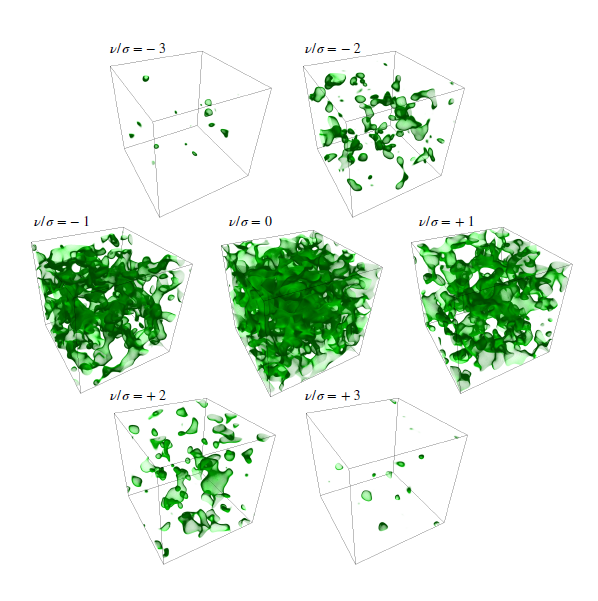
\includegraphics[width=0.6\textwidth]{figures/boundaries.png}
    \caption{Example of an excursion set and its boundary for a field for a smoothed three-dimensional Gaussian field.}
    \label{fig:level_set_example}
\end{figure}

The motion-invariants are defined as the integrals of the Minkowski functionals over the excursion set $S_{\nu}$, are d+1 and are called the Minkowski functionals. For a 2-dimensional map, these are:

\begin{itemize}
    \item $M_0(S_{\nu})$: the area of the excursion set, which is the integral of the field over the set $S_{\nu}$.
    \item $M_1(S_{\nu})$: the perimeter of the excursion set.
    \item $M_2(S_{\nu})$: the Euler characteristic of the excursion set, which is a measure of the connectivity of the set.
\end{itemize}

From these, we can define a lot of properties that can be calculated to characterize the structures in Orion A and B. 

The following section is divided into two parts: global properties and local properties. Global properties are those that describe the overall structure of the ISM, while local properties are those that describe how the structure changes as a function of column density.

\section{Global Properties}

% Add interpretation (D=2, D=1)
% Add longer explaination on Lovejoy thoughts
\subsection{Global Fractal Dimension}

The fractal dimension is a measure of the border complexity of a given structure. This can be calculated using the Minkowski functionals, specifically the perimeter and area \cite{cannon1984fractal}. 
The main idea for this approach is that, for a given border length, a simple border will always enclose a larger area than a complex border.

On this idea, the perimeter-area relation is defined as:

\begin{equation}
    \label{eq:perimeter_area}
    P = A^{\frac{D}{2}}
\end{equation}

By measuring the perimeter $P$ and area $A$ of a structure at different thresholds and fitting the log of the perimeter to the log of the area, we can derive the fractal dimension $D$ of the overall structure. 

If the linear fit is good, then one can argue that the structure has no characteristic scale, and thus behaves as a fractal. An example of this can be seen in Figure \ref{fig:perimeter_area_example}, where data from meteological clouds was used to derive the fractal dimension of the structure. The slope of the linear fit gives the fractal dimension of the structure, which is a measure of its complexity. The lack of a characterstic scale is evident from the linear fit, hinting at turbulent processes that are responsible for the formation of the structure.

\begin{figure}[t]
    \centering
    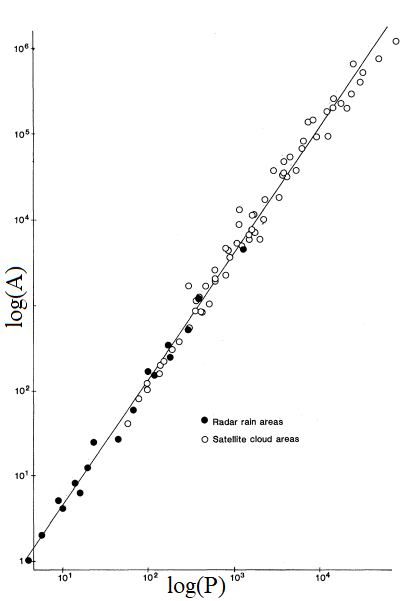
\includegraphics[width=0.4\textwidth]{figures/lovejoy.png}
    \caption{Example of the perimeter-area relation for meteorological clouds \cite{lovejoy1982area}. The slope of the linear fit gives the fractal dimension of the structure.}
    \label{fig:perimeter_area_example}
\end{figure}

This counts in this work a global property of the cloud.

The perimeter-area relation is a powerful tool for analyzing the complexity of structures in the ISM. It's simple, yet effective, and can be applied to a wide range of structures, from clouds to galaxies. The fractal dimension derived from the perimeter-area relation can provide insights into the physical processes that shape these structures, such as turbulence, gravity, and magnetic fields. It is also powerful to analyze the evolution of structures as a function of column density threshold.
However, it is important to note that the perimeter-area relation is not always applicable to all structures. Furthermore, numerical effects can also play a role in the calculation of the fractal dimension, as we will see in the simulations section. Artifacts also have an effect on this method \cite{imre2006artificial}. This is to say, that the method has its limitations and simulations play an important role in understanding these effects. 

\section{Local Properties}

\subsection{Local Fractal Dimension}

One other advanatge of the perimeter-area relation is that it can be inverted to derived the fractal dimension of a structure at a given column density threshold. By inverting the relation \ref{eq:perimeter_area}, we can derive the local fractal dimension $D$ as a function of the column density threshold $\nu$:

\begin{equation}
    \label{eq:local_fractal_dimension}
    D(\nu) = 2 \times \frac{\log(P(\nu))}{\log(A(\nu))}
\end{equation}

This opens up a lot of possibilities to analyze the structures in the Orion Molecular Cloud, as we can calculate $P(\nu)$ and $A(\nu)$ for different structures in different ways. At each column density thresholds, we can calculate the perimeters and areas of all of the structures in the map, and calculate the local fractal dimension for that specific threshold by summing over all of the structures. An example of this can be seen in Figure \ref{fig:local_fractal_dimension_example}, where perimeters and areas of structures are calculated at a column density threholds.

Conversely, we can also calculate the local fractal dimension for each structure, and analyze how the fractal dimension changes as a function of column density threhold.

\begin{figure}[t]
    \centering
    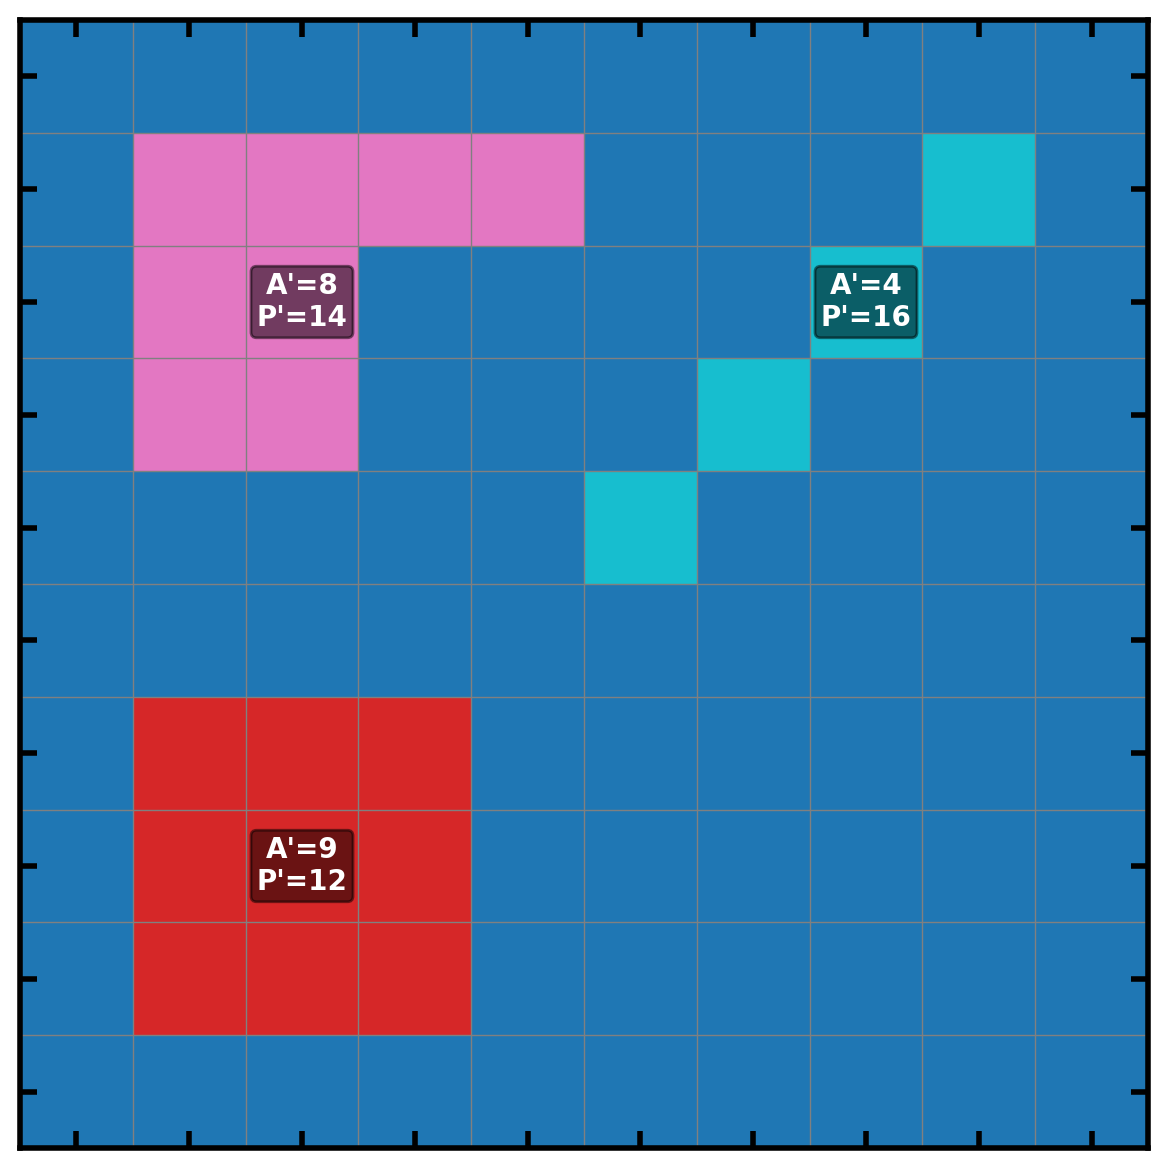
\includegraphics[width=0.5\textwidth]{figures/example_calculations.png}
    \caption{Simplified example of the calculation of perimeters and areas of structures at a given column density threshold. The local fractal dimension can be calculated by summing over all of the structures at that threshold, or for each of the single structures.}
    \label{fig:local_fractal_dimension_example}
\end{figure}

\subsection{Dendrograms}

To this end, the segmentation of structures with a dendrogram appraoch is useful.

\subsection{Mass-Size-Fractal Dimension (MSD) plane}

Since it is possible to calculate the local fractal dimension for single structure, we can connect this property to more physical aspects of the substructures, namely mass and size. This then allows us to include new information on mass-size diagrams, creating a Mass-Size-Fractal Dimension (MSD).

The dendrogram-like segmentation is an important aspect of this process, as it ensures a proper characterization and recognition of the sub-structures. 

% maybe also as a 3d plane?

\subsection{Euler characteristic}

Euler characteristic, often denoted as $\chi$ or $M_2(S_{\nu})$, and in two dimensions it is given by:
\begin{equation}
    \chi = \text{Number of connected regions} - \text{Number of holes}
\end{equation}
For a given excursion set $S_{\nu}$, the Euler characteristic provides a measure of the topology of the structures, indicating how many isolated regions and holes are present at a specific threshold. In practice, a positive Euler characteristic indicates more isolated regions than holes, while a negative value suggests a topology dominated by holes.

The Euler characteristic is closely related to the genus $G$ of the structure, where in two dimensions $G = 1 - \chi$. The genus is commonly used in cosmology and astrophysics to describe the connectivity of structures, such as the filamentary network in the ISM or the cosmic web. By analyzing the Euler characteristic or genus as a function of the threshold, one can gain insights into the morphological transitions and connectivity of the observed structures.

\section{Connection to star formation}

TBD

\section{Simulations}

\subsection{Simulation for the global properties}

\subsection{Simulations fotr the local properties}

GRF, simple shapes, etc.

\section{Uncertainties}

\subsection{Perimeter and Area}

\subsection{Map's}
